
%
% raspberry p3 spec: https://www.raspberrypi.org/magpi/raspberry-pi-3-specs-benchmarks/

\section{Embedded Computing Platform Comparison}\label{sec:comparison}


\begin{table*}[h]
  \centering
  \begin{adjustbox}{width=1\textwidth}
  \begin{tabular}{|c|c|c|c|}
    \hline
    Item    & Raspberry Pi 3 (B)   & Intel UP                  & NVIDIA Jetson TX2\\
    \hline
            & BCM2837              & X5-Z8350 (Cherry Trail)   & Tegra X2 \\
    CPU     & 4x Cortex-A53@1.2GHz/512KB L2  &
              4x Atom@1.92GHz/2MB L2 &
              4x Cortex-A57@2GHz/2MB L2 \\
            &              &              & 2x Denver@2.0GHz/2MB L2 (not used)  \\
    \hline
    GPU     &  VideoCore IV (not used)    &
               Intel HD 400 Graphics (not used) &
               Pascal 256 CUDA cores   \\
    \hline
    Memory  & 1GB LPDDR2   &  2GB DDR3L     & 8GB LPDDR4              \\
    \hline
	Peak Memory Bandwidth & 8.5 GB/s & 12.8 GB/s & 59.7 GB/s \\
	\hline
	Measured Bandwidth & 2127.94 MB/s & 3951.94 MB/s & 4447.90 MB/s \\
	\hline
	Cost (\$) & 35 & 100 & 600 \\
	\hline
  \end{tabular}
  \end{adjustbox}
  \caption{Compared embedded computing platforms}
  \label{tbl:platforms}
\end{table*}

In this section, we compare three computing platforms---the Raspberry
Pi 3, the Intel UP~\footnote{http://www.up-board.org/up/} and the NVIDIA
Jetson
TX2~\footnote{http://www.nvidia.com/object/embedded-systems-dev-kits-modules.html}---from
the point of view of supporting end-to-end deep learning
based autonomous vehicles. 
Table~\ref{tbl:platforms} shows architectural features of the three
platforms~\footnote{The GPU of Intel UP and the two Denver cores in the
  Tegra TX2 are not used in evaluation due to TensorFlow issues.}.
  
Our basic approach is to use the same DeepPicar software, and repeat
the experiments in Section~\ref{sec:evaluation} on each hardware
platform and compare the results. 
%We do not, however, repeat the cache
%partitioned experiments done on the Pi 3, as we did not believe our 
%findings warranted further experimentation on additional platforms. 
For the Jetson TX2, we have two different system configurations,
which differ in whether TensorFlow is configured to use its GPU or
only the CPU cores. Thus, a total of four system configurations are
compared.

\begin{figure}[h]
  \centering
  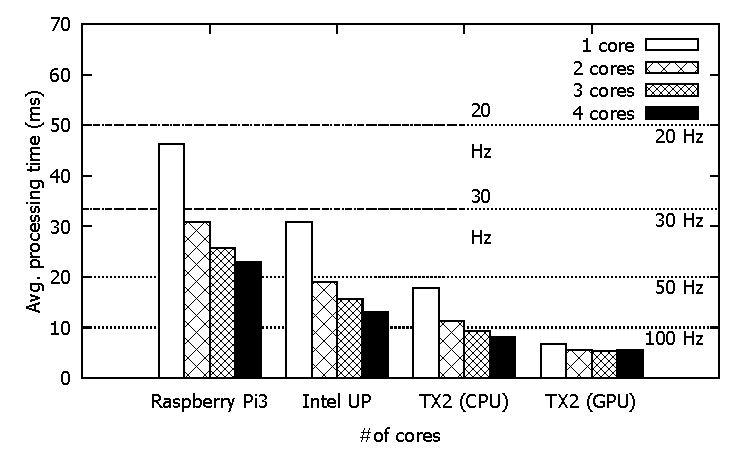
\includegraphics[width=.7\textwidth]{figs/compare_core}
  \caption{Average control loop execution time.} 
  \label{fig:sys_core}
\end{figure}

Figure~\ref{fig:sys_core} shows the average control loop completion
timing of the four system configurations we tested as a function of
the number of CPU cores used.
First, both the Intel UP and Jetson TX2 exhibit superior performance when
compared with the Raspberry Pi 3. 
When all four CPU cores are used, the Intel UP is 1.33X faster than
the Pi 3, while the TX2 (CPU) and TX2 (GPU) are 2.79X and 4.16X times faster,
respectively, than the Pi 3. 
As a result, they are all able to satisfy the 33.$\overline{\mbox{33}}$ ms 
WCET by a clear margin,
%%  (in the worst case, the UP Board would 
%% still meet it by $\sim$20 ms) --> where's the data showing this?
and, in the case of the TX2, 50 Hz or even 100 Hz real-time control is
feasible with the help of its GPU. Another observation is that the TX2
(GPU) performance does not change much, as most of the neural network 
computation is done at the GPU.

\begin{figure}[h]
  \centering
  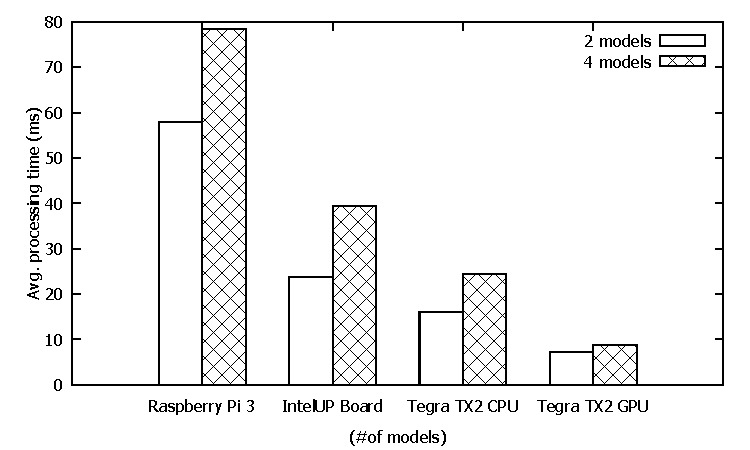
\includegraphics[width=.7\textwidth]{figs/compare_model}
  \caption{Average control loop execution time when multiple DNN
    models are co-scheduled. }
  \label{fig:sys_model}
\end{figure}

The Intel UP board and Jetson TX2 also perform much better when multiple DNN models
are co-scheduled. Figure~\ref{fig:sys_model} shows the results of the
multi-model co-scheduling experiment. Once again, they can comfortably
satisfy 30 Hz real-time performance for all of the co-scheduled DNN control
loops, and in the case of the TX2 (GPU), 100 Hz real-time control is still
feasible. Given that the GPU must be shared among the co-scheduled DNN
models, the results suggest that the TX2's GPU has sufficient capacity to
accomodate multiple instances of the DNN models we tested.

\begin{figure}[h]
  \centering
  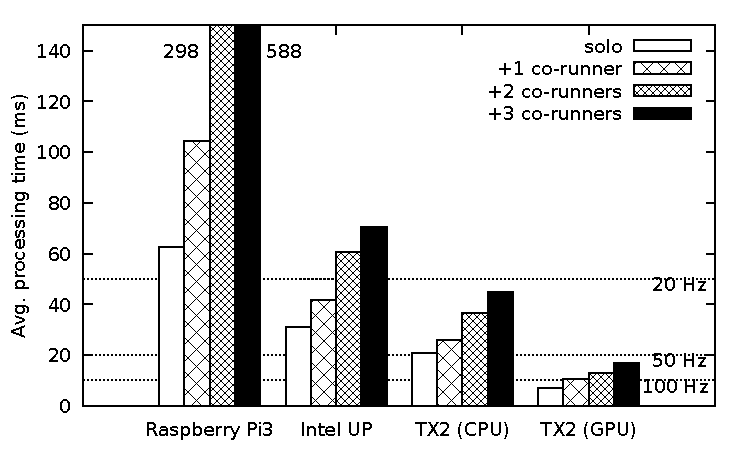
\includegraphics[width=.7\textwidth]{figs/compare_benchmark}
  \caption{Average control loop execution time in the presence of an
    increasing number of memory intensive applications on idle CPU cores.}
  \label{fig:sys_bench}
\end{figure} 

\begin{figure}[h]
  \centering
  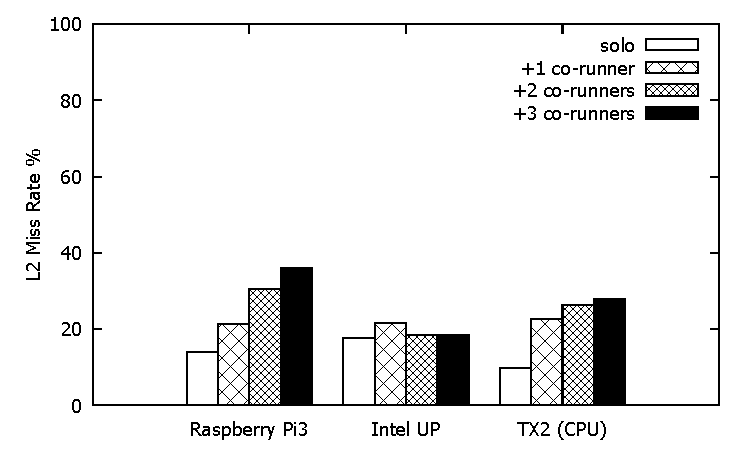
\includegraphics[width=.7\textwidth]{figs/compare_l2missrate}
  \caption{L2 miss rates in the presence of an increasing number of 
			memory intensive applications on idle CPU cores.}
  \label{fig:sys_l2miss}
\end{figure}

Finally, we compare the effect of co-scheduling memory bandwidth
intensive synthetic benchmarks on the DNN control loop timing. 

Figure~\ref{fig:sys_bench} shows the results. As discussed in 
Section~\ref{sec:eval-memhog}, we observed dramatic execution time
increases, up to 11.6X, in Raspberry Pi 3 as we increased the number of
co-scheduled tasks. We also observe increased control loop execution
timing in the Intel Up and Jetson TX2, but the degree of the increase is 
not as dramatic as the Pi 3. Compared to their respective solo timings 
(i.e., the model runs on a single core in isolation), Intel UP suffers up to
2.3X execution time increase; TX2 (CPU) and TX2 (GPU) suffer up to
2.2X and 2.1X increases, respectively. This is somewhat surprising
because the Raspberry Pi 3's cores are in-order architecture based while
the cores in the Intel Up and NVIDIA TX2 are out-of-order architecture
based, and that the memory intensive tasks on out-of-order cores can
generate more memory traffic. We believe that this is because the
memory subsystems in the Intel UP and TX2 platforms provide higher
performance than the memory subsystem of the Pi 3 as suggested from
the measured memory bandwidth results in Table~\ref{tbl:platforms}
('Measured Bandwidth').

Another interesting observation is that the TX2 (GPU) also suffers
considerable execution time increase (2.1X) despite the fact that the
co-scheduled synthetic tasks do not utilize the GPU. In other words,
the DNN model has dedicated access to the GPU. This is, however, a
known characteristic of integrated CPU-GPU architecture based
platforms where both CPU and GPU share the same memory
subsystem~\cite{Ali2017}. As a result, the TX2 (GPU) fails to meet the
10ms deadline for 100 Hz control that would have been feasible if
there was no contention between the CPU cores and the GPU.

Figure~\ref{fig:sys_l2miss} shows the L2 miss rates of DNN control
loop. The key takeaway of this result is that the L2 miss rate is a
poor indicator to the execution time of the control loop. As shown
already, the Raspberry Pi 3's increased L2 misses do not fully explain
increases in processing times. In case of the Intel UP, as the number of
interfering Bandwidth benchmark instances increases, the L2 miss rates
even drop slightly. In case of the TX2 (CPU), from solo to one co-runner,
L2 miss rate increase almost twice, but then the execution time
increase is a little less than 10\%. However, when there are
co-runners, even though the L2 miss rates are largely unchanged, the
DNN processing time increases significantly. The TX2 (GPU) also shows
similar behavior. All of these results essentially point to the fact
that DNN inferencing workload is largely memory performance sensitive
but not L2 cache space sensitive. 

%% However, the L2 miss rates of the Pi 3 and TX2 platforms follow the same expected 
%% pattern, as can be seen in Figure~\ref{fig:sys_l2miss}. Namely, the 
%% percentage of L2 miss rates increases are more 
%% memory intensive co-runners are introduced. This was not the case for 
%% the UP board, where the model running on two cores generated the highest
%% percentage of L2 cache misses. This is most likely due to the CPU 
%% architecture of the UP's CPU which is Intel based, whereas both the Pi 3
%% and TX2 have ARM based CPUs.


In summary, we find that today's embedded computing platforms, even as
inexpensive as a Raspberry Pi 3, are powerful enough to support
vision and end-to-end deep learning based real-time control
applications. Furthermore, availability of CPU cores and GPU on these
platforms allow consolidating mutiple deep neural network based AI
workloads. However, shared resource contention among these diverse
computing resources remains an important issue that must be understood
and controlled, especially for safety-critical applications.
